\documentclass[10pt,psamsfonts]{amsart}

%-------Packages---------
\usepackage{amssymb,amsfonts}
%\usepackage[all,arc]{xy}
\usepackage{enumerate}
%\usepackage{mathrsfs}
\usepackage{subcaption}
\usepackage{graphicx}
\usepackage{caption}
\usepackage[margin=0.3in]{geometry}

%--------Theorem Environments--------
%theoremstyle{plain} --- default
\newtheorem{thm}{Theorem}[section]
\newtheorem{cor}[thm]{Corollary}
\newtheorem{prop}[thm]{Proposition}
\newtheorem{lem}[thm]{Lemma}
\newtheorem{conj}[thm]{Conjecture}
\newtheorem{quest}[thm]{Question}

\theoremstyle{definition}
\newtheorem{defn}[thm]{Definition}
\newtheorem{defns}[thm]{Definitions}
\newtheorem{con}[thm]{Construction}
\newtheorem{exmp}[thm]{Example}
\newtheorem{exmps}[thm]{Examples}
\newtheorem{notn}[thm]{Notation}
\newtheorem{notns}[thm]{Notations}
\newtheorem{addm}[thm]{Addendum}
\newtheorem{exer}[thm]{Exercise}

\theoremstyle{remark}
\newtheorem{rem}[thm]{Remark}
\newtheorem{rems}[thm]{Remarks}
\newtheorem{warn}[thm]{Warning}
\newtheorem{sch}[thm]{Scholium}

\makeatletter
\let\c@equation\c@thm
\makeatother
\numberwithin{equation}{section}

\bibliographystyle{plain}

%--------Meta Data: Fill in your info------
%\title{Homework 1}

%\author{Won I. Lee}

%\date{July 30, 2016}


\begin{document}
	
%\maketitle

\begin{center}
	{\bf Homework 2}
\end{center}

\section{Logistic Regression}

We begin by investigating the effects of regularization ($L_1$ and $L_2$) on logistic regression classifiers. That is, we consider loss functions of the following form:
$$E_{LR}(w, w_0) \equiv NLL(w, w_0) + \lambda\|w\|_k^k$$
where $k = 1, 2$, and $NLL$ is the negative log-likelihood loss for logistic regression. We note that such classifiers can be trained efficiently via gradient descent, with the gradient term being given by (using $L_2$ as an example):
$$\frac{\partial E_{LR}}{\partial dw_j} = \frac{\partial NLL}{\partial dw_j} + \lambda \frac{\partial \|w\|_k^k}{\partial w_j} = \left\{ \begin{matrix} -\sum_i \frac{y^{(i)} e^{-y^{(i)}(wx^{(i)} + w_0)}}{1 + e^{-y^{(i)}(wx^{(i)} + w_0)}} & j =0 \\ -\sum_i \frac{y^{(i)} x^{(i)}_j e^{-y^{(i)}(wx^{(i)} + w_0)}}{1 + e^{-y^{(i)}(wx^{(i)} + w_0)}} + 2\lambda w_j & j \neq 0 \end{matrix}  \right.$$
To explore the effects of regularization, we first consider the non-regularized case, with $\lambda = 0$. {\bf Figure 1(a)} shows that, as expected, the magnitude of the weight vector goes to infinity as the number of iterations of gradient descent grows large. (For the purposes of illustration, we used a deliberately small step size, $\eta = 10^{-4}$.) Even when we include $L_2$ regularization at $\lambda = 1$, the magnitude of the weight vector diverges, indicating that the regularization is not strong enough to counteract the tendency of logistic regression to yield large weights towards a step function. However, when we add regularization terms of size $\lambda = 5, 10$, the weights stabilize at a finite value, with higher regularization yielding lower-magnitude weights, as expected.

To understand the impact of using $L_1$ compared to $L_2$ regularization, we conduct a systematic analysis of how the weights of the logistic regression model behave under each method. We vary values of $\lambda$ and fit our model to 4 artificial 2D datasets using both regularization methods, and provide results from dataset 1 for illustrative purposes. {\bf Figure 1(b)-(d)} demonstrates our results. In terms of classification accuracy (Figure 1(b)), we see that regardless of regularization strength ($\lambda$), the $L_2$-regularized model yields near-perfect performance on both training and validation. However, the $L_1$-regularized model drops to random chance (i.e. accuracy is 50\%) after a certain threshold $\lambda$. This is explained by Figure 1(c) and (d), which shows that beyond these threshold values of $\lambda$, the weight vector becomes essentially 0, so the model does not learn anything under $L_1$ regularization. This result is in line with our intuition about $L_1$ regularization, as it is known to yield sparse weight vectors. Figure 1(d) especially demonstrates this phenomenon, in which both $w_1$ and $w_2$ go to 0 after $\lambda \approx 400$ for $L_1$ but $w_2$ remains nonzero even at $\lambda \geq 1000$ for $L_2$.

{\bf Figure 2} further illuminates this idea by depicting the decision boundaries of the regularized logistic regression models. We see that when $\lambda$ is small, both $L_1$ and $L_2$ regularization yield reasonable decision boundaries that obtain perfect classification of all points. On the other hand, for $\lambda =10$, both regularization schemes yield a flatter decision boundary, with partial classification error. However, the $L_2$-regularized model yields a slightly non-zero sloped boundary that is able to capture some of the classification features, whereas the sparsity from $L_1$ yields a very flat boundary that leads to lower accuracy.

Finally, we examine which regularizer yields the best performance in terms of classification accuracy on an unseen test set, when the regularization strength is selected based on validation. We find that this choice depends strongly on the dataset. For example, on datasets 1 and 2, in which the training and validation sets are rather similar, the $L_1$ regularizer with modest $\lambda$ strength of $0.01$ fares best on the validation set. Unfortunately, the lack of complete separability on the test set yields lower accuracy for dataset 2. On the other hand, for dataset 3, there are a number of points in the validation set that are misclassified (high $x_1$, lower $x_2$) if the boundary is fit too closely to the training set, so a higher $\lambda$ value is favored, which yields higher accuracy on the test set. Finally, nonsensical values are given for dataset 4, which is highly not linearly separable.

\begin{figure}[b]
	\centering
	\begin{subfigure}[b]{0.23\textwidth}
		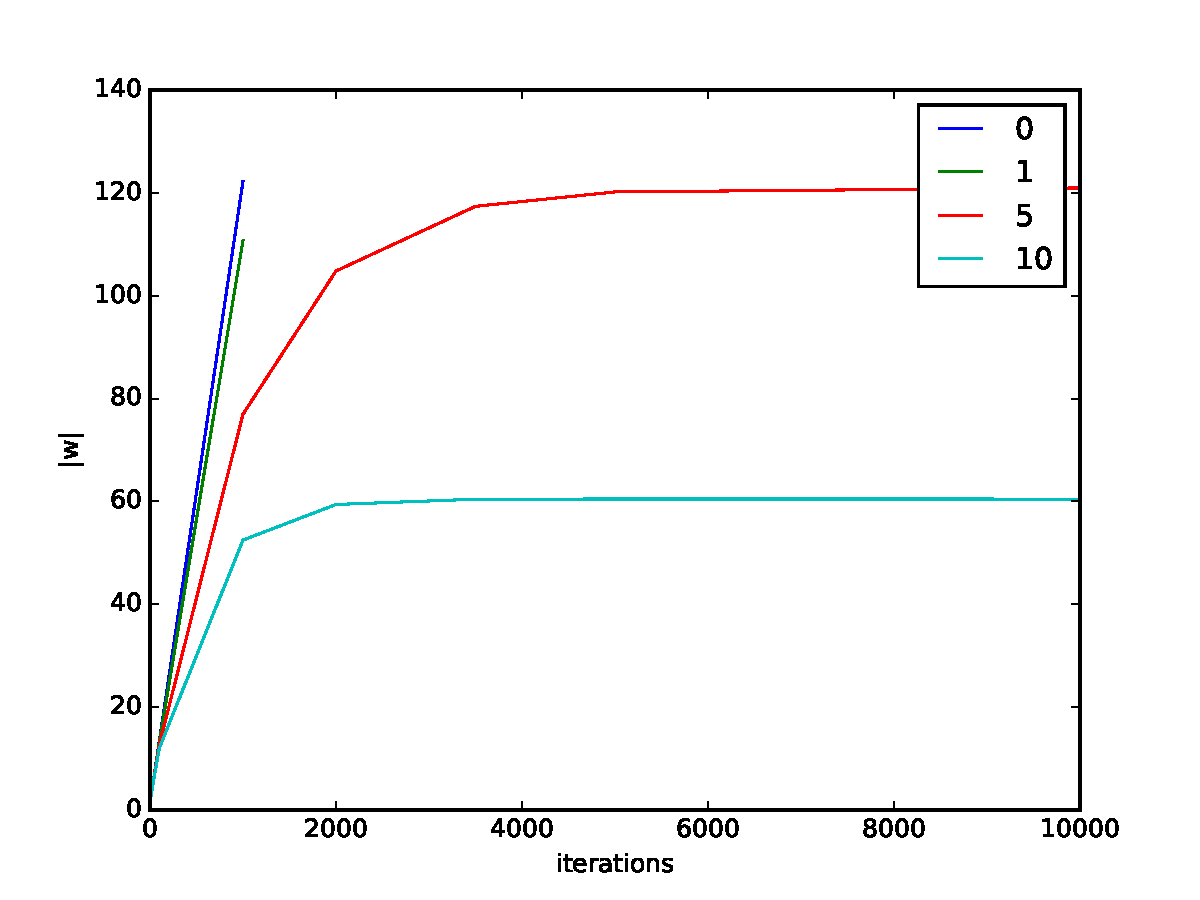
\includegraphics[width=\textwidth]{hw2_1-1_1.pdf}
		\caption{}
	\end{subfigure}
	\begin{subfigure}[b]{0.23\textwidth}
		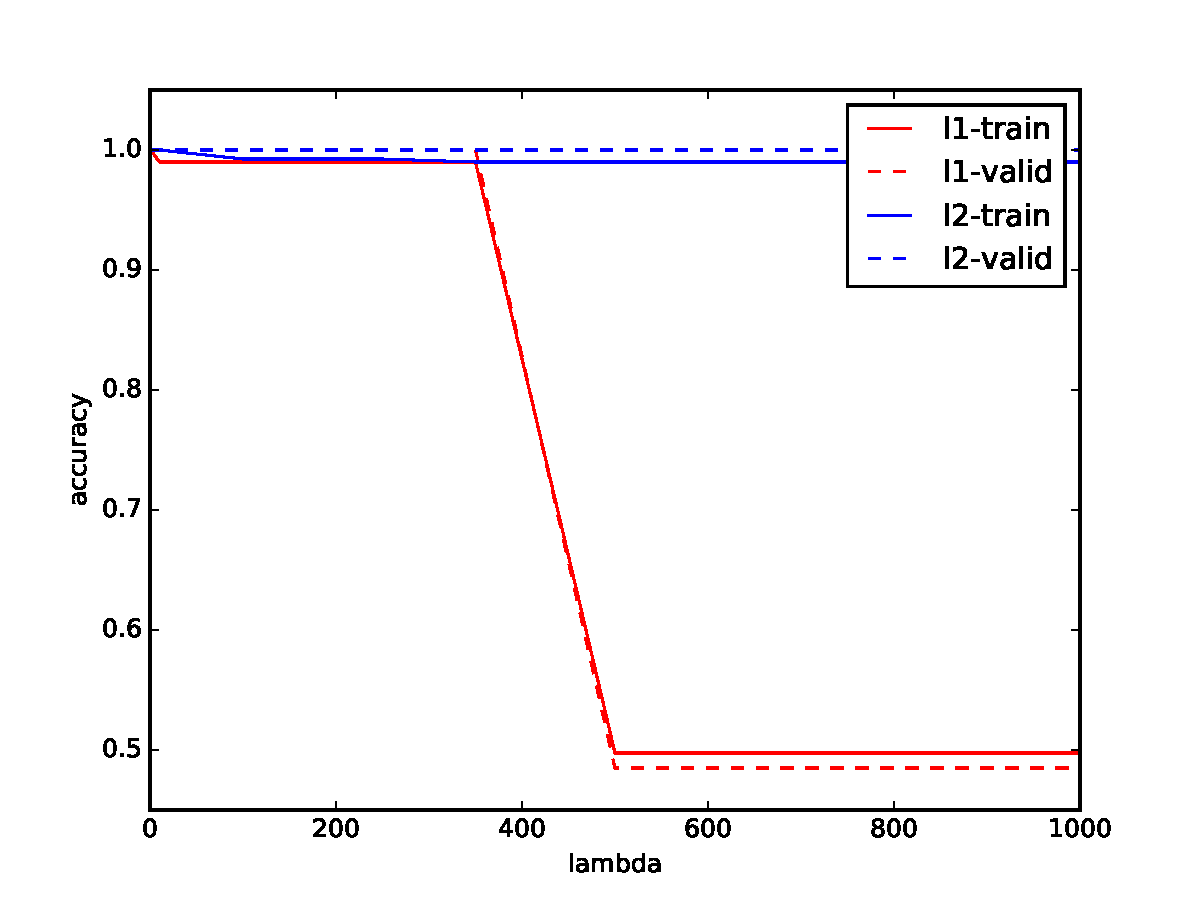
\includegraphics[width=\textwidth]{hw2_1-2_1.pdf}
		\caption{Accuracy}
	\end{subfigure}
	\begin{subfigure}[b]{0.23\textwidth}
		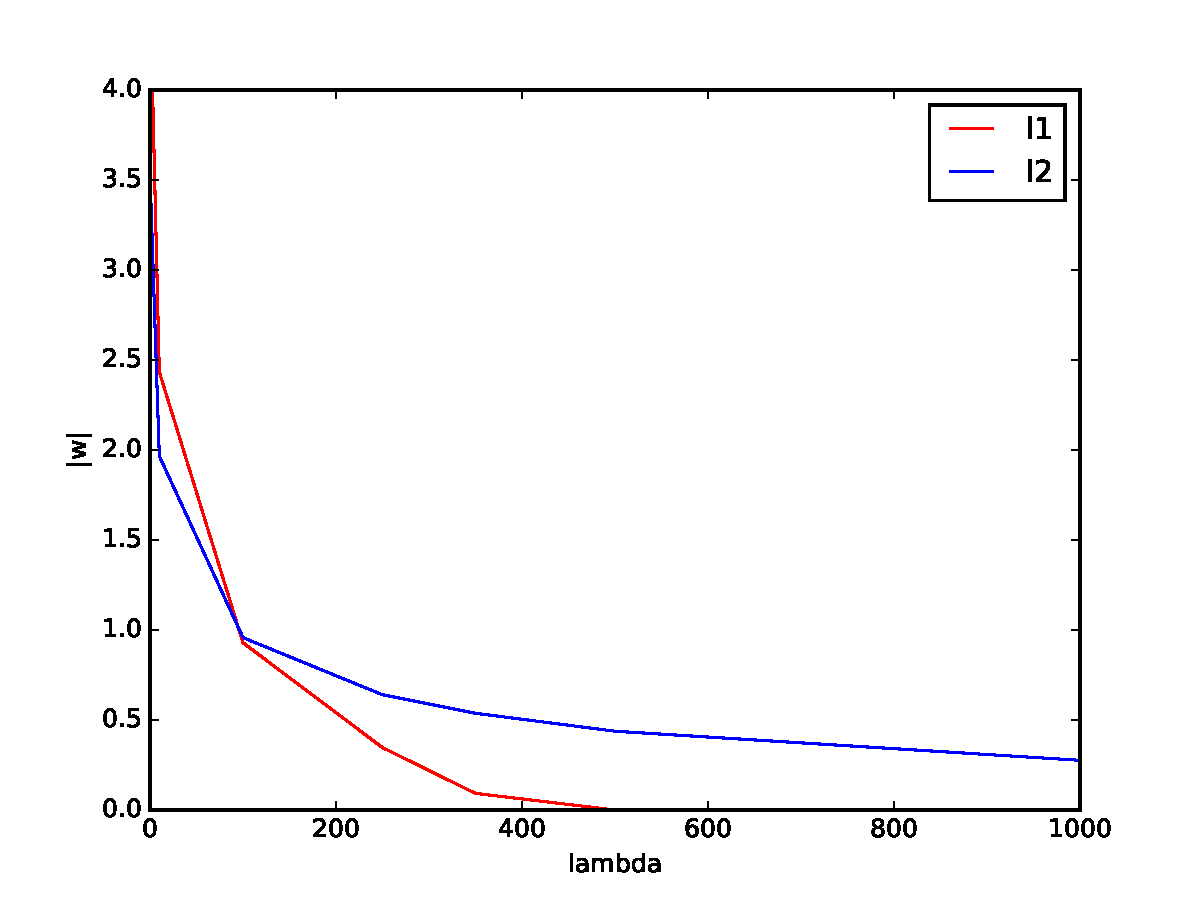
\includegraphics[width=\textwidth]{hw2_1-2_2.pdf}
		\caption{$\|w\|_2$}
	\end{subfigure}
	\begin{subfigure}[b]{0.23\textwidth}
		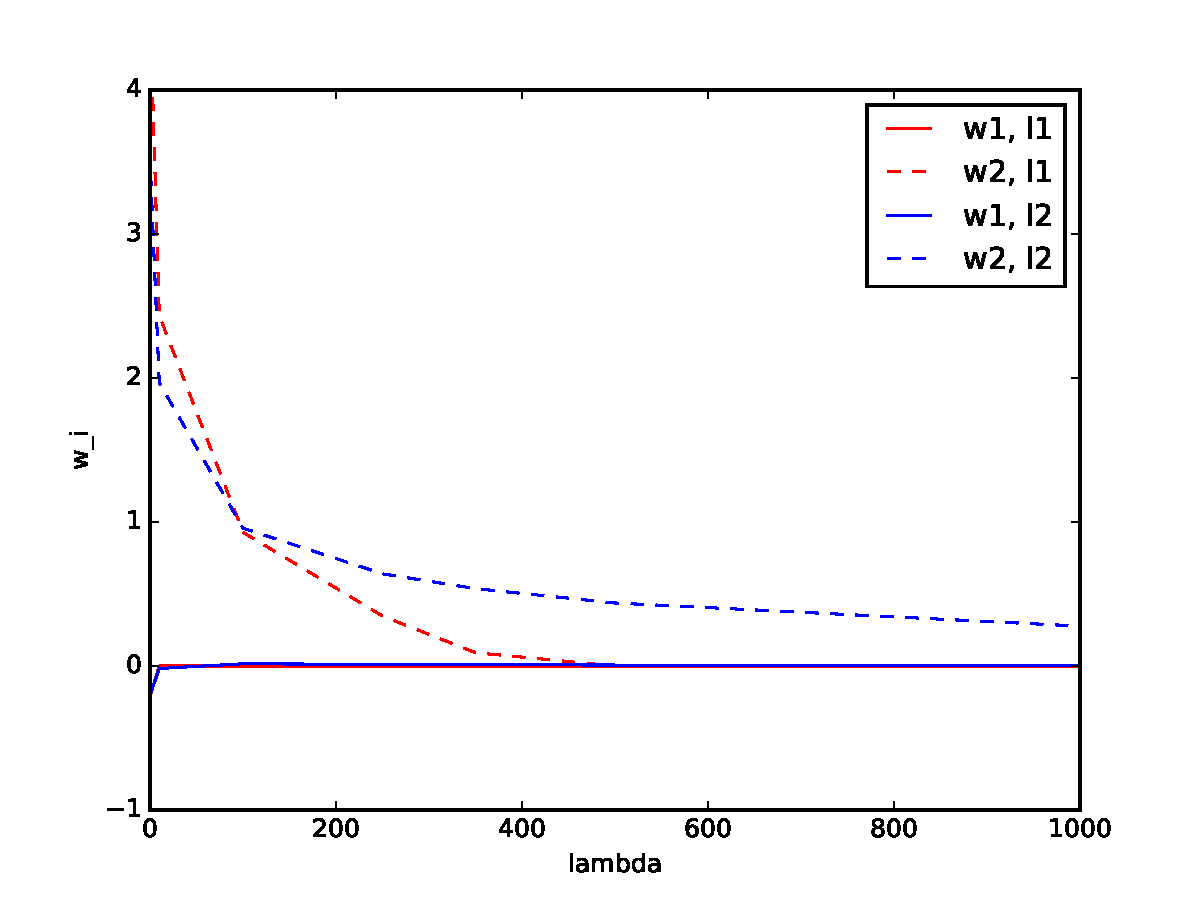
\includegraphics[width=\textwidth]{hw2_1-2_3.pdf}
		\caption{$w_1, w_2$}
	\end{subfigure}
	\caption{Effects of regularization on the weights (coefficients) of logistic regression model for various values of $\lambda$, and under $L_1$ vs. $L_2$ regularization.}
\end{figure}

\begin{figure}
	\centering
	\begin{subfigure}[b]{0.23\textwidth}
		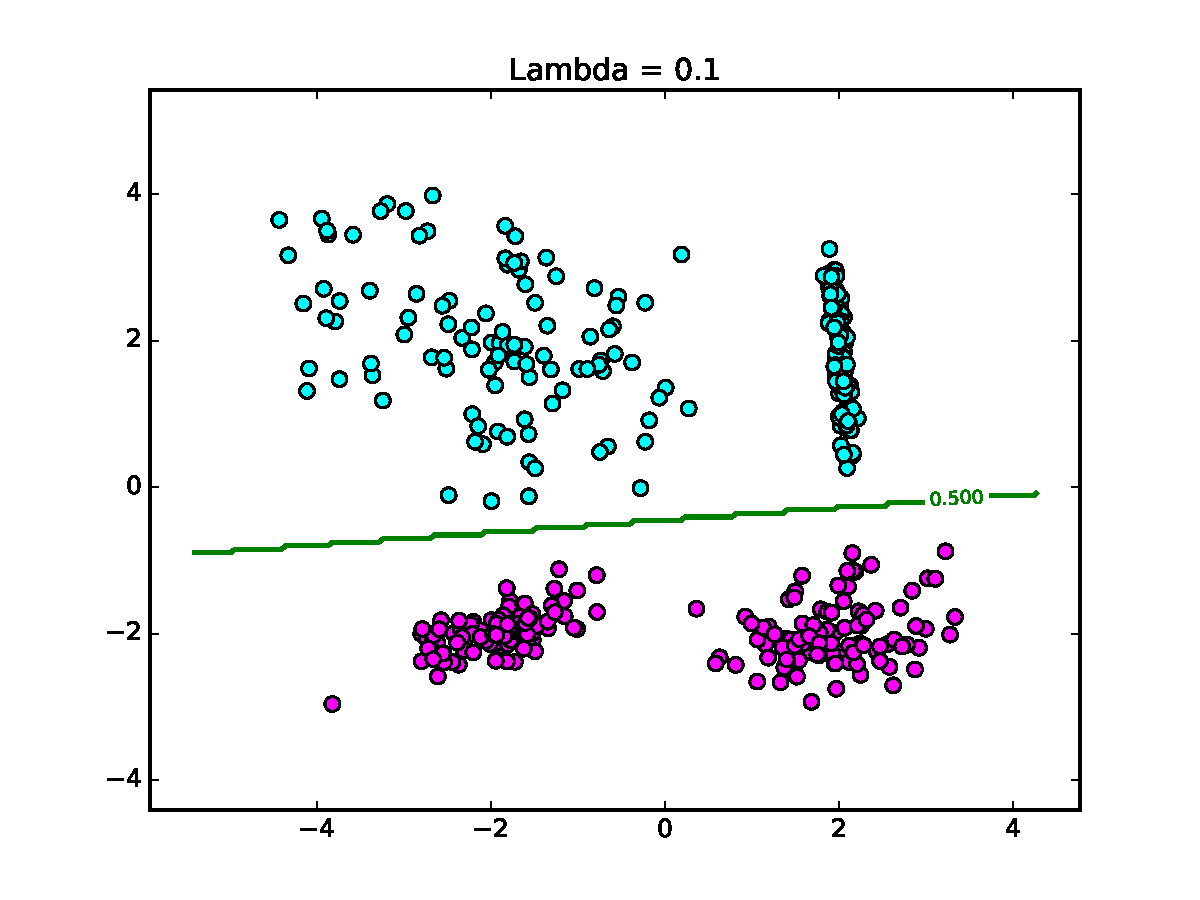
\includegraphics[width=\textwidth]{hw2_1-2_4.pdf}
		\caption{$L_1, \lambda = 0.1$}
	\end{subfigure}
	\begin{subfigure}[b]{0.23\textwidth}
		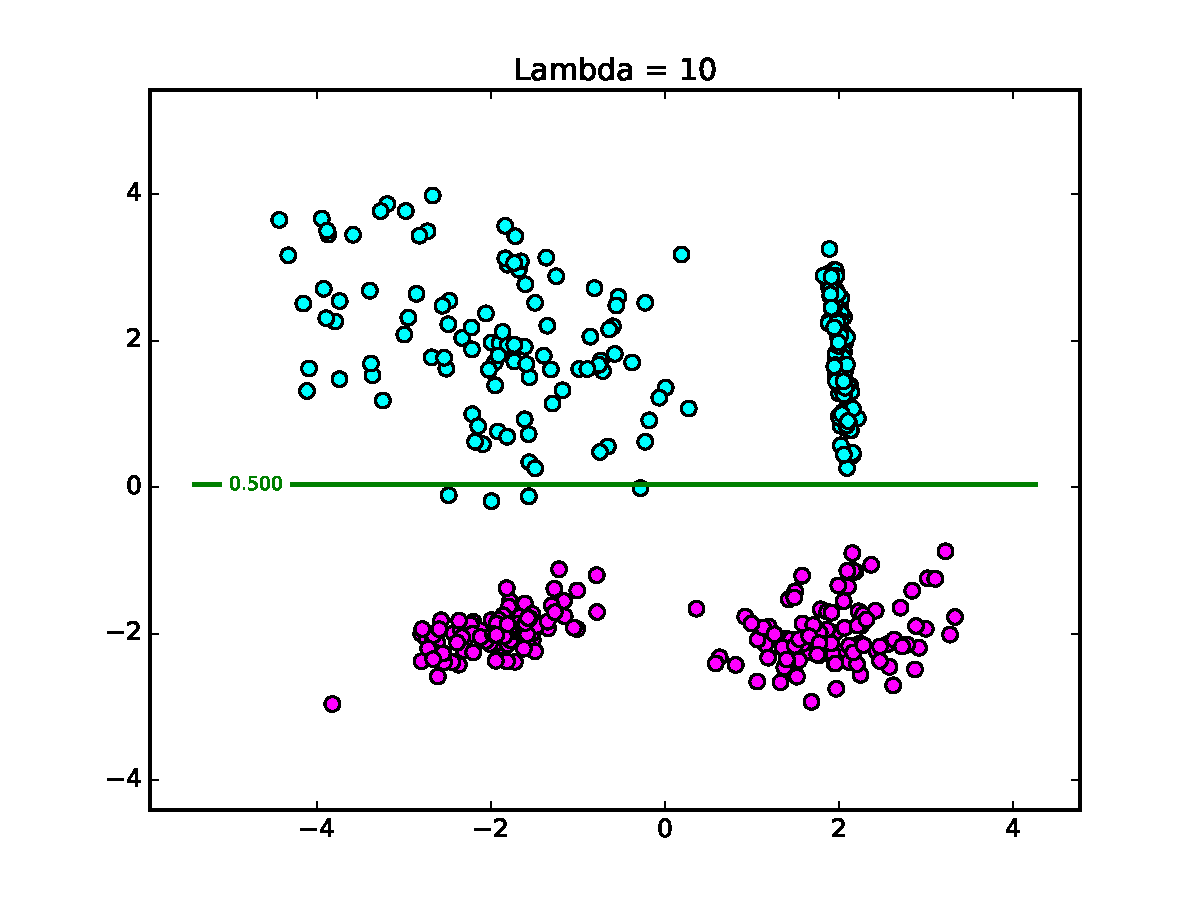
\includegraphics[width=\textwidth]{hw2_1-2_6.pdf}
		\caption{$L_1, \lambda = 10$}
	\end{subfigure}
	\begin{subfigure}[b]{0.23\textwidth}
		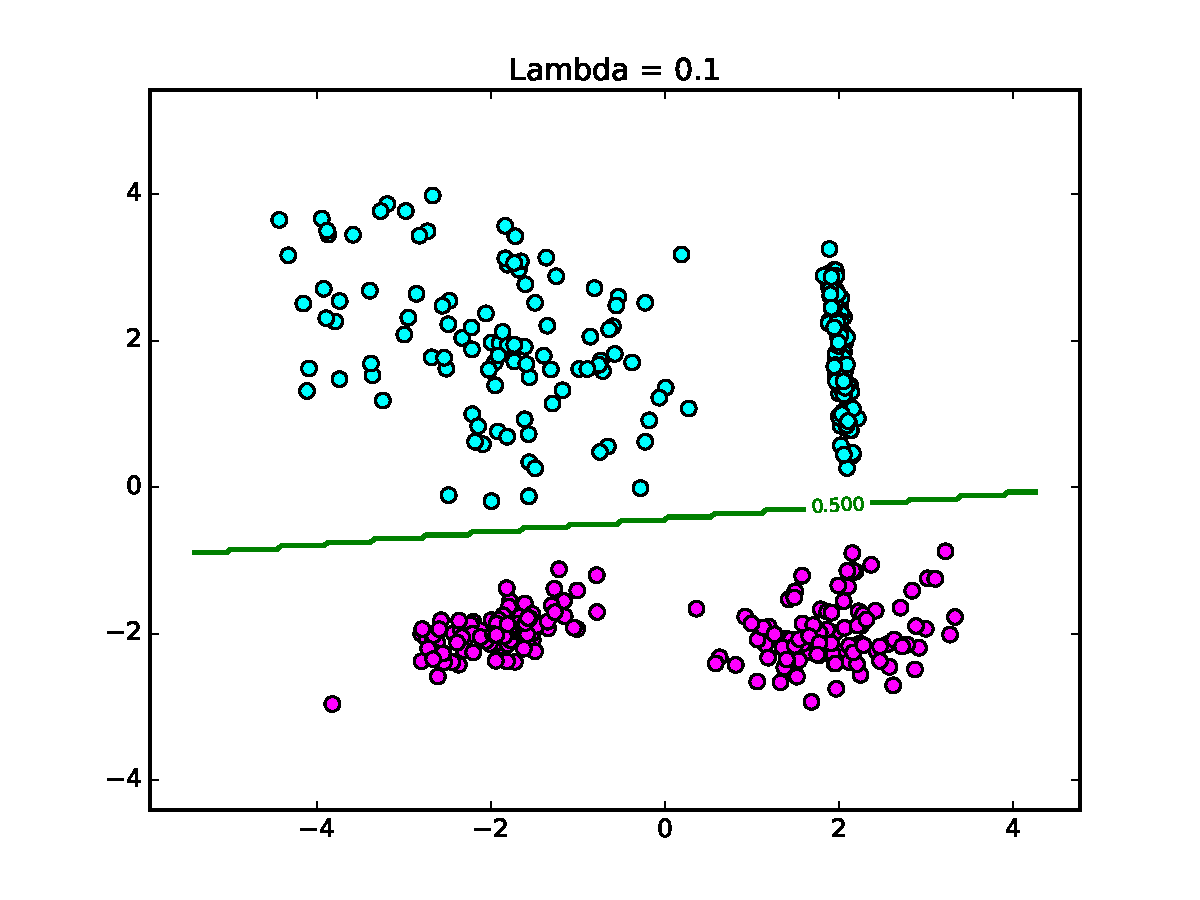
\includegraphics[width=\textwidth]{hw2_1-2_8.pdf}
		\caption{$L_2, \lambda = 0.1$}
	\end{subfigure}
	\begin{subfigure}[b]{0.23\textwidth}
		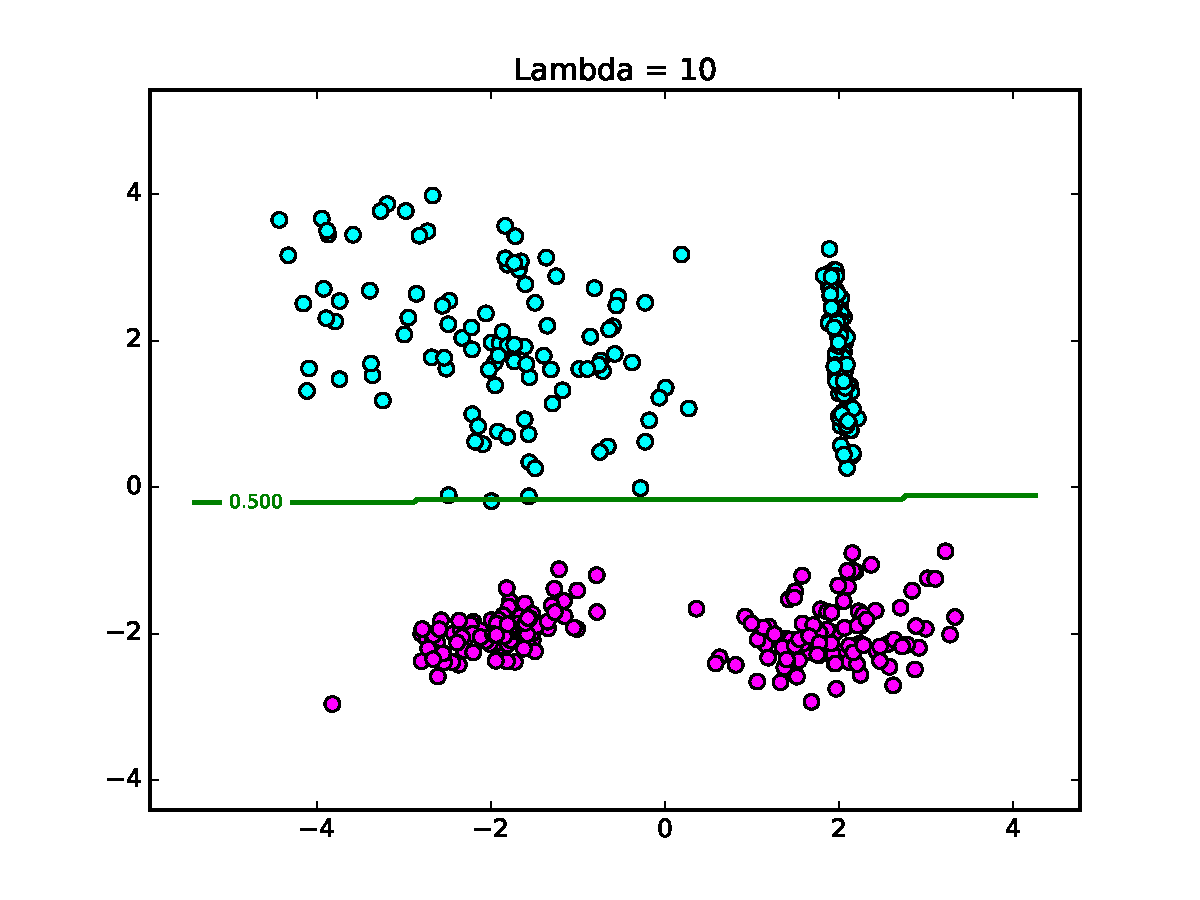
\includegraphics[width=\textwidth]{hw2_1-2_10.pdf}
		\caption{$L_2, \lambda = 10$}
	\end{subfigure}
	\caption{Decision boundaries for the training set for artificial dataset 1, for $L_1$ vs $L_2$ regularization.}
\end{figure}

\begin{figure}
	\centering
	\begin{subfigure}[b]{0.4\textwidth}
		\centering
		\begin{tabular}{c|c|c|c}\hline
			Dataset & Regularizer & $\lambda$ & Accuracy\\\hline
			1 & $L_1$ & 0.01 & 1 \\
			2 & $L_1$ & 0.01 & 0.805\\
			3 & $L_2$ & 0.3& 0.96  \\
			4 & $L_1$ & 100& 0.5 \\\hline
		\end{tabular}
		\caption{Regularizer and $\lambda$ Values}
	\end{subfigure}
	\begin{subfigure}[b]{0.35\textwidth}
		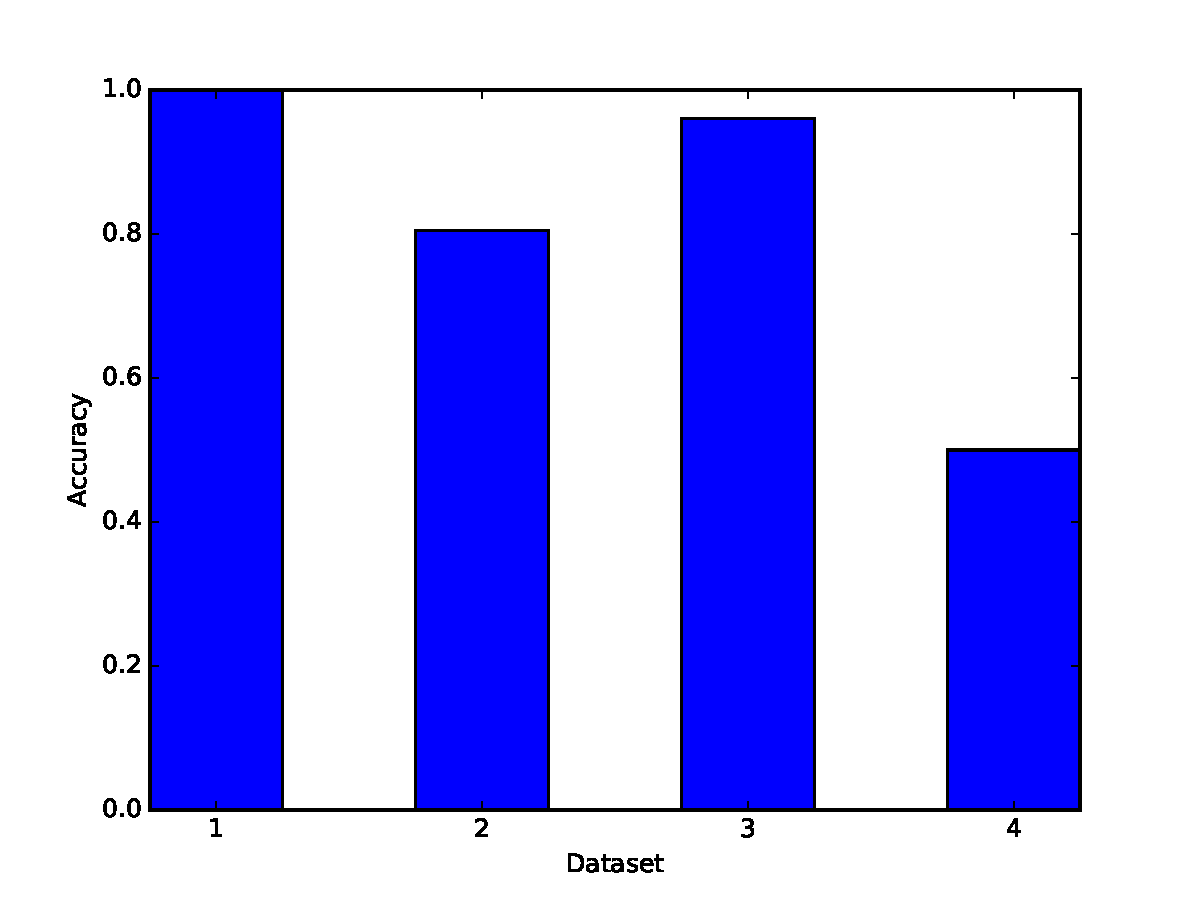
\includegraphics[width=\textwidth]{hw2_1-3_1.pdf}
		\caption{Accuracy}
	\end{subfigure}
	\caption{Best-performing regularizers and $\lambda$ values for each artificial dataset (selected on validation), with classification accuracy on corresponding test set.}
\end{figure}

\section{Support Vector Machine}

\section{Support Vector Machine with Pegasos}

\section{Handwritten Digit Recognition with MNIST}













In this section, we investigate the performance of gradient descent-based algorithms for minimizing scalar functions of vector arguments. In particular, we consider the following functions: 1) the negative Gaussian function:
$$f(x) = -\frac{1}{\sqrt{(2\pi)^n |\Sigma|}} \exp\left[ -\frac{1}{2}(x-u)^T\Sigma^{-1}(x-u) \right]$$
and 2) the quadratic bowl function $f(x) = \frac{1}{2}x^TAx - x^Tb$.
\subsection{Initialization and Hyperparameters} We first explore the batch gradient descent algorithm. For loss function $f(x)$, the gradient descent algorithm performs $x = x - \eta \nabla f(x)$
where $\eta$ is the step size. These iterations continue until a convergence threshold is met, i.e. $|f(x) - f(\tilde{x})| < \epsilon$, where $x, \tilde{x}$ are successive iterations. We investigate the dependence of this algorithm on the initialization of the algorithm as well as its hyperparameters, namely the step size $\eta$ and the convergence threshold $\epsilon$. Throughout the experiments, we fix the following parameters of the functions $u = (10, 10),\Sigma = \begin{pmatrix} 1000 & 0 \\ 0 & 1000\end{pmatrix}$ and $A = \begin{pmatrix} 10 & 5 \\ 5 & 10\end{pmatrix},b = (400, 400)$.

First, we note that the large variance in the negative Gaussian density yields small objective function values (scaled by the reciprocal of the determinant of $\Sigma$), as well as small gradients. Thus, we consider only large step sizes that will yield noticeable increments in the values of $x$; otherwise, no learning is achieved. Similarly, we only consider very small $\epsilon$ for the same reasons.

The results are shown in {\bf Figure 1} for the negative Gaussian function, where the $z$-axis is the squared distance. We have used step sizes of $10^5, 10^6, \dots, 10^10$ and convergence criteria of $10^{-10}, 10^{-11}, \dots, 10^{-20}$. The plots reveal two major points. First, for any choice of initialization and step size used in the experiments, gradient descent does not converge to a suitable solution until $\epsilon$, the convergence threshold, is sufficient small. As the plots demonstrate, we require $\epsilon \approx 10^{-15}$ or $\log(\epsilon) \approx -35$ before the squared error falls to negligible values. Second, the step size must bee sufficiently large before convergence is achieved, in the same vein as the convergence threshold. Even for suitable $\epsilon$ values, a relatively small step size (i.e. $10^5$) does not yield approximate convergence to the correct solution. Indeed, for most cases, we require a step size of $\eta \approx 10^7$ before the suared loss becomes negligible. As discussed above, these issues are germane to the negative Gaussian function, due to the large determinant value effectively annihilating the step sizes unless sufficiently large.

On the other hand, the quadratic bowl function does not have such issues, and using large step sizes generally yields divergence. Indeed, even using $\eta = 1$ leads to diverging estimates for $\epsilon \approx 10^{-15}$. Thus, for this case we consider step sizes of $10^{-1}, 10^{-2}, \dots, 10^{-5}$ and similarly convergence criteria of $10^{-10}, 10^{-11}, \dots, 10^{-20}$. Results as shown in {\bf Figure 2} demonstrate a very similar behavior for the quadratic bowl function; the convergence threshold $\epsilon$ must be suitably small for convergence to the correct values. In this case, however, if the step size $\eta$ is too small, then no $\epsilon$ used in our experiments can yield convergence, unlike the case of the negative Gaussian, in which a suitably small $\epsilon$ would yield convergence in all step sizes. We must have a large enough step size (in this case $\eta \approx 0.01$) for convergence in this example.


\end{document}


